\section{روش‌های متداول پردازش سیگنال}
در بخش \ref{ch:background} در مورد نحوه تصویر برداری \mri صحبت شد و دیدم که نمونه ها از فضای فوریه تصویر برداشته می‌شوند که آن فضا \kspace نام‌دارد. اما تصویر در نهایت یک تصویر حقیقی است و نه مختلط و موهومی، بنابراین می‌توان از این خاصیت استفاده کرد تا تعداد اخذ نمونه را به 50 درصد کاهش داد. البته در این روش باعث می‌شود که \lr{SNR} کم تر شود که در مورد آن نیز صحبت خواهد شد.

\begin{قضیه}[فوریه توابع حقیقی]\label{th:F-real}
اگر یک تابع حقیقی $s(x,y)$ در احتیار داشته باشیم در این صورت داریم:
$$S(k_x, k_y) = \F[s(x,y)](k_x, k_y) \; \Rightarrow \; S(k_x, k_y) = S^*(-k_x,-k_y) $$
\end{قضیه}

بنابراین طبق قضیه \ref{th:F-real}
می‌توان این طور گفت که توابع حقیقی در حوزه فوریه (\kspace)
تقارن 180 درجه دوران دارند. این یعنی گوشه بالا سمت راست \kspace با گوشه پایین سمت چپ تصویر برابر است.





\begin{figure}[t!]
	\centering
	\begin{copyrightBox}{0.7\linewidth}{\doiSource{10.1017/CBO9780511545405}}
	\centering
	\subfigure[]{
		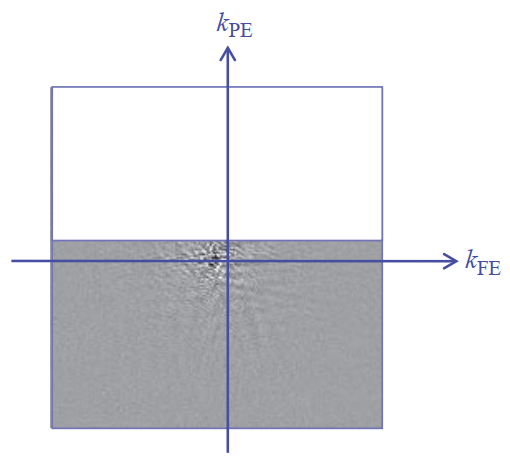
\includegraphics[width=0.35\linewidth]{chapters/chapter-3/figs/half-fourier-ud}
		\label{subfig:half-fourier-ud}	
	}
	\hspace{0.15\linewidth}
	\subfigure[]{
		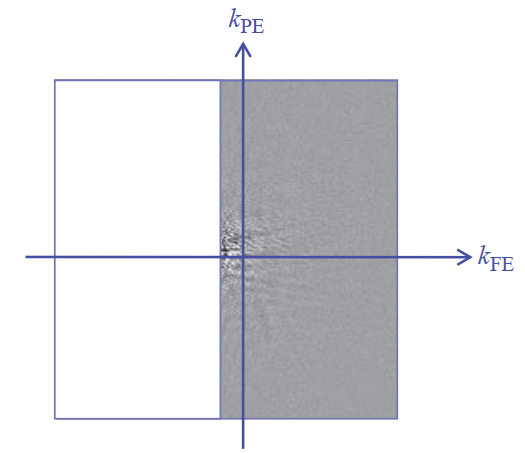
\includegraphics[width=0.35\linewidth]{chapters/chapter-3/figs/half-fourier-rl}
		\label{subfig:half-fourier-rl}	
	}	
	\end{copyrightBox}
	\removevspace[1]
	\caption{}
	\label{fig:half-fourier}
\end{figure}



از این تکنیک به نام های «نیم فوریه \LTRfootnote{half Fourier}»، «نیم‌اسکن \LTRfootnote{halfscan}» و یا «نیم نکس \LTRfootnote{half NEX}» نیز یاد می‌شود. در هرکدام، صرفا کمی بیشتر از نصفی از دادگان اخذ می‌شود.  در واقع توسط این روش نصف گام های گرادیان کد‌کردن فاز حذف می‌شود. در مورد \kspace نیز می‌توان گفت که مانند شکل \ref{subfig:half-fourier-ud} صرفا نیمه پایینی(یا بالایی) فضا را اخذ می‌کنیم و نیمه بعدی را با توجه به قضیه‌‌ی \ref{th:F-real} از آن نیمه، باز سازی می‌کنیم. به قضیه‌ \ref{th:F-real}، \textit{ساخت مزدوج}
\LTRfootnote{conjugate synthesis}
نیز گفته می‌شود. 

هر چند با این تکنیک تقریبا 50 درصد از لحاظ زمانی صرفه جویی می‌شود و خیلی روی رزولوشن مکانی تاثیر نمی‌گذارد، اما تقریبا 30 درصد \lr{SNR} را کاهش می‌دهد.\cite{McRobbie} برای درک بهتر این موضوع، توجه داشته باشید که درست است که از لحاط تئوری نیمه بالایی \kspace از نیمه پایینی بدست می‌آید اما هردو نیمه دو نویز ناهمبسته حس می‌کنند که این اتفاق باعث می‌شود اطلاعات این دو نیمه باهم متفاوت باشد. در حقیقت \lr{SNR} با ضریب
 $\frac{1}{\sqrt{2}}$
کاهش پیدا میکند و این مقدار کاهش برابر با
 $1-\frac{1}{\sqrt{2}}= 0.2928$
می‌باشد. بنابراین این روش هرچند سادگی ریاضیاتی خاص خود را دارد اما باعث کاهش \lr{SNR} می‌شود و باید به دنبال روش های مناسب تری بود که از اطلاعات بیشتری استفاده کنند.




